\section{Fundamental of Push Pull Converter}
The half-bridge converter is a DC-DC power converter topology designed for medium-power applications, combining efficiency, simplicity, and galvanic isolation. Its core structure consists of two switching devices (MOSFETs or IGBTs) arranged in a half-bridge configuration across a DC input. The input voltage ($V_\text{in}$) is split by two series capacitors ($C_1$ and $C_2$), each charged to $\frac{V_\text{in}}{2}$, ensuring balanced voltage distribution.
\begin{figure}[h!]
    \centering
    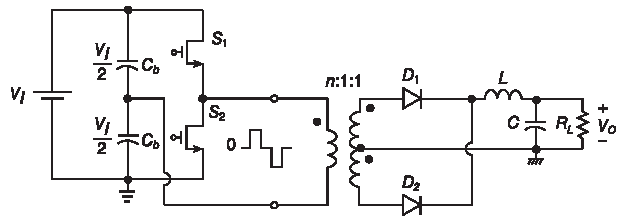
\includegraphics[width=0.9\linewidth]{Pictures/report_img/circuit_haft_bridge.pdf}
    \caption{\textcolor{blue}{\textit{\footnotesize  Haft-Bridge Converter}}}
\end{figure}

\subsection{Basic Working Principle}
The half-bridge converter is a versatile DC-DC converter topology used for medium-power applications. Its operation relies on alternating switching states to transfer energy through a transformer while maintaining galvanic isolation. Below is a breakdown of its basic operation and working principle :
\subsubsection{Switch 1 ON and Switch 2 OFF}
\begin{itemize}
    \item Current path: \( S_1 \) → Transformer primary → \( C_2 \).
    \item Primary voltage: \( +V_{\text{in}}/2 \).
    \item Magnetizing current increases in transformer core.
\end{itemize}
\begin{figure}[h!]
    \centering
    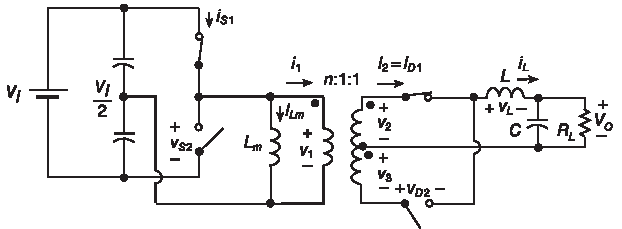
\includegraphics[width=0.9\linewidth]{Pictures/report_img/s1_closed_s2_open.pdf}
    \caption{\textcolor{blue}{\textit{\footnotesize  Switch 1 ON and Switch 2 OFF}}}
\end{figure}
\subsubsection{Switch 1 OFF and Switch 2 ON}
\begin{itemize}
    \item Current path: \( C_1 \) → Transformer primary → \( S_2 \)
    \item Primary voltage: \( -V_{\text{in}}/2 \)
    \item Magnetizing current decreases/reset
\end{itemize}
\begin{figure}[h!]
    \centering
    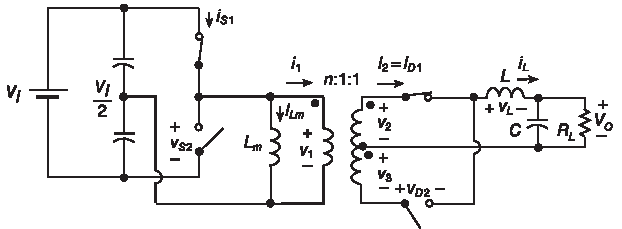
\includegraphics[width=0.9\linewidth]{Pictures/report_img/s1_closed_s2_open.pdf}
    \caption{\textcolor{blue}{\textit{\footnotesize Switch 1 OFF and Switch 2 ON}}}
\end{figure}
\subsubsection{Dead Time}
\begin{itemize}
    \item Short delay between switching transitions to prevent shoot-through.
    \item Ensures only one switch conducts at a time
\end{itemize}
\subsection{Energy Transfer and Output Regulation}
\subsubsection{Transformer Action}
\begin{itemize}
    \item Alternating \( \pm V_{\text{in}}/2 \) pulses induce AC voltage in secondary.
    \item Voltage scaled by turns ratio \( N_p:N_s \)
\end{itemize}
\subsubsection{Output Voltage Equation}
\[
V_{\text{out}} = \frac{V_{\text{in}}}{2} \cdot \frac{N_s}{N_p} \cdot D
\]
\newpage
\subsection{Haft-Bridge Converter CCM Waveform}
\begin{figure}[h!]
    \centering
    
\includegraphics[width=1\linewidth]{Pictures/report_img/ccm_waveform.pdf}
    \caption{\textcolor{blue}{\textit{\footnotesize  Waveforms in the half-bridge converter with a transformer center-tapped rectifier for CCM.}}}
\end{figure}
